\documentclass[twoside,openright]{report}
\usepackage[utf8]{inputenc}

\usepackage{graphicx}
\usepackage{hyperref}

\begin{document}


{\Huge Points }\\
\rule{12cm}{0.05cm}\\
\newline
\newline
We start by plotting some points on the graph (1, 2), (-3, 4), (4, -3), (-3, -4), (4, 0), (0, 4).
As we can see the point (5, 4) lies in 1st quadrant, (-3, 4) lies in second quadrant, (-3, -4) lies in third quadrant, (4, -3) lies in fourth quadrant, (4, 0) is on the X axis and (0, 4) is on the Y axis.\\
This particular image is from Desmos. So if you want you can try it out here \url{https://www.desmos.com/calculator/dtraqcrzqt}.\\
\begin{figure}[h!]
  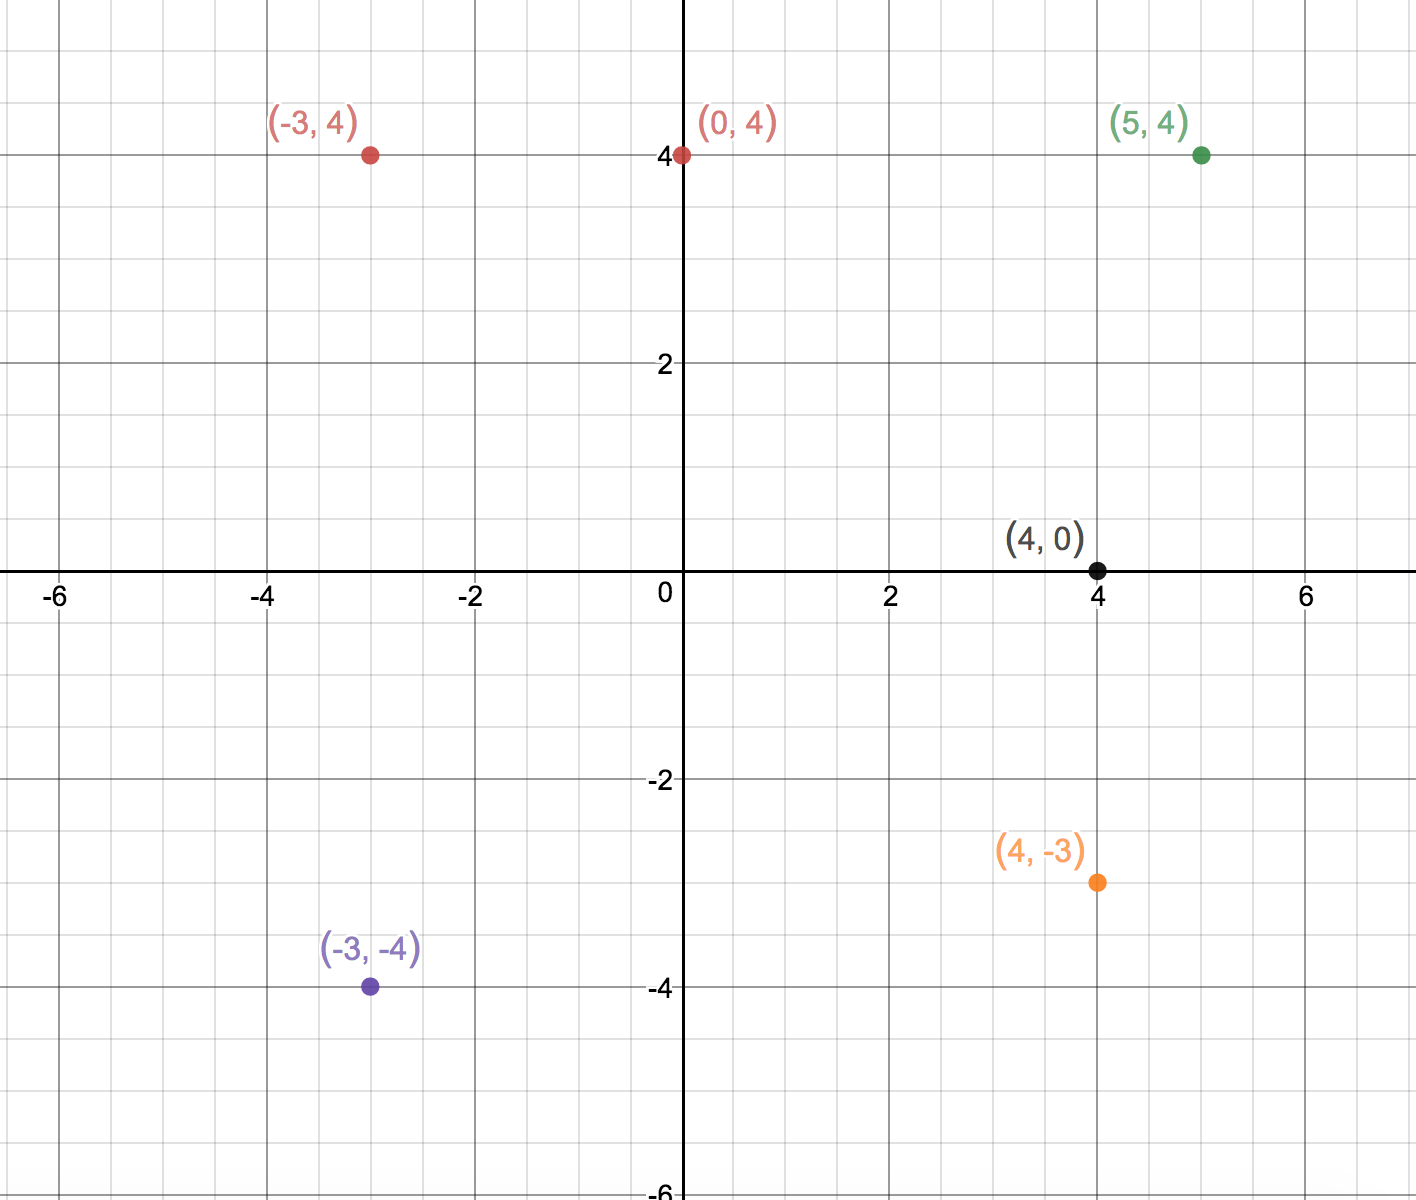
\includegraphics[width=\linewidth]{img/image2.png}
  \caption{Plotting points.}
  \label{fig:axis1}
\end{figure}
\clearpage
\pagenumbering{roman} 
 \setcounter{page}{2}
 %Page i%
\end{document}